\section{Problem No.1} \label{sec:prob2}
\subsection{Problem Description:} 
In one spatial dimension the linearized equations of acoustics (sound waves) are
$$
p_{t} + Ku_{x}=0\\
\rho u_{t}+p_{x}=0
$$
where $u$ is the velocity and $p$ is the pressure, $\rho$ is the density, and $K$ is the bulk modulus.
\begin{enumerate}
\item Show that this system is hyperbolic and find the wave speeds.
\item Write a program to solve this system using \protect{\lw} in original variables on (0,1) using a cell centered grid $x_{j}=(j-\frac{1}{2})\Delta x$ for $j=1...N.$ Write the code to use ghost cells, so that different boundary conditions can be changed by simply changing the values in the ghost cells. Ghost cells are cells outside the domain whore values can be set at the beginning of a time step so that code for updating cells adjacent to the boundary is identical to the code for interior cells.
Set the ghost cells at the left by 
$$
p_{0}^{n}=p_{1}^{n}\\
u_{0}^{n}=-u_{1}^{n}
$$
and set the ghost cells on the right by
$$
p_{N+1}^{n} = \frac{1}{2}(p_{N}^{n}+u_{N}^{n}\sqrt{K\rho})\\
u_{N+1}^{n} = \frac{1}{2}(\frac{p_{N}^{n}}{\sqrt{K\rho}} + u_{N}^{n})
$$
Run simulations with different initial conditions. Explain what happens at the left and right boundaries. 
\item Give a physical interpretation and a mathematical explanation of these boundary conditions

\end{enumerate}


\subsection{Solution:} 
\paragraph{Part 1:} To prove that the system in hyperbolic, we start by writing the system of equation in matrix. Thus,

$$
q_{t} + A q_{x}=0
$$

\begin{bmatrix} 
p\\
u
\end{bmatrix}_{t}
+
\begin{bmatrix} 
0 & K\\
1/\rho & 0
\end{bmatrix}
\begin{bmatrix} 
p\\
u
\end{bmatrix}_{x}
=
\begin{bmatrix} 
0\\
0
\end{bmatrix}

For the above system, we need to prove that $A$ is diagonalizable and  its eigenvalues are real and distinct (strictly hyperbolic). Since the transpose of $A$ is a diagonal matrix, then $A$ is diagonalizable. The eigenvalues of $A$ can be obtain by solving the following 
$$
Det(A-\lambda I)=0\\
\lambda^{2}=\frac{K}{\rho}\\
\lambda_{1,2} = \pm \sqrt{\frac{K}{\rho}}
$$

$K$ is the bulk modulus which measure how incompressible a substance is which always positive (ration of infinitesimal pressure increase to resulting relative decrease in volume). $\rho$ is density which always positive. Thus, the $\lambda$ is real and distinct which makes the eigenvalues of $A$ real and distinct. Thus, the system is (strictly) hyperbolic. 

\paragraph{Part 2:} 
The system of equations above can be discretized using \protect{\lw} and it become
$$
p_{j}^{n+1} = p_{j}^{n} - \frac{K \Delta t}{2 \Delta x}(u_{j+1}^{n}-u_{j-1}^{n}) + \frac{K^{2} \Delta t^{2}}{2 \Delta x ^{2}}(u_{j-1}^{n}-2u_{j}^{n}+u_{j+1}^{n})\\
u_{j}^{n+1} = u_{j}^{n} - \frac{ 1/\rho \Delta t}{2 \Delta x}(p_{j+1}^{n}-p_{j-1}^{n}) + \frac{(1/\rho)^{2} \Delta t^{2}}{2 \Delta x ^{2}}(p_{j-1}^{n}-2p_{j}^{n}+p_{j+1}^{n})
$$

We used Courant number ($\nu$) of $0.8$ from which we can compute the time step $\Delta t$ such that $\Delta t= \frac{\nu \Delta x}{|\lambda|}$, where $\lambda$ is the speed of sound (according to Newton-Laplace). %We take $K=101kPa$ and $\rho=1.225 kg/m^3$ for air in ordinary conditions which gives speed of sound to be $287.139m/s$ which is close to the ideal value for dry air ($343 m/s$).

We used four different initial conditions; sine wave, triangular function, mixed sine wave and triangular function and exponentially decaying sine wave. Figures \ref{fig:sol_sin}, \ref{fig:sol_tri}, \ref{fig:sol_sin_tri} and \ref{fig:sol_sin_expo} show the obtained solution at different time intervals up to time = 1 second. 

For the run tests with different initial conditions, we observed that the initial conditions starts by splitting in two parts (waves) one moves to the right and the other moves to the left (as shown in Figures \ref{fig:sol_sin}, \ref{fig:sol_tri}, \ref{fig:sol_sin_tri} and \ref{fig:sol_sin_expo}). Due to the given boundary conditions, the right side absorbs the incoming wave while the left side reflects/bounces the incoming wave which travel all the way to the right side which in turn absorbs it. 


      
\begin{figure}[]
 \centering     
   \subfloat [0 sec]{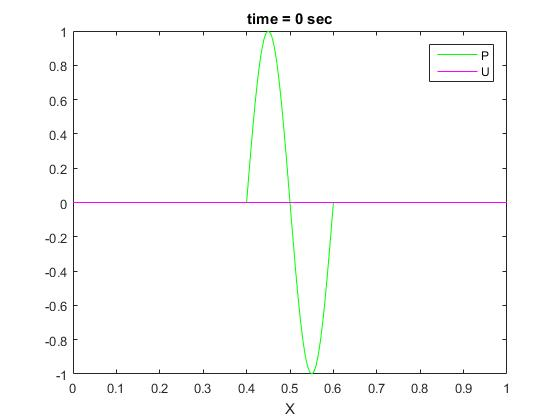
\includegraphics[width=0.3\textwidth]{fig/p1/sin_0.jpg}}
   \subfloat [0.2 sec]{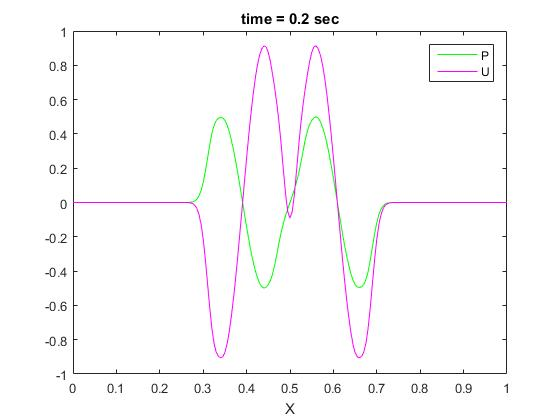
\includegraphics[width=0.3\textwidth]{fig/p1/sin_0p2.jpg}}
   \subfloat [0.4 sec]{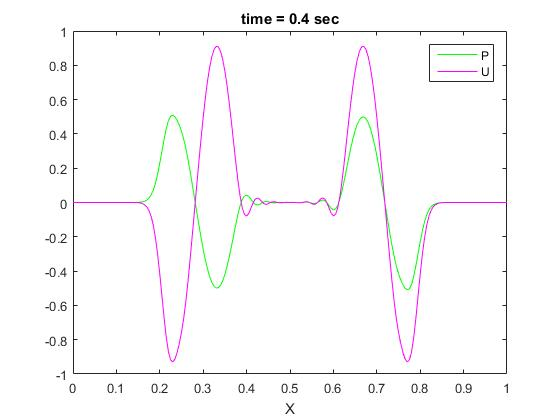
\includegraphics[width=0.3\textwidth]{fig/p1/sin_0p4.jpg}}
   
   \subfloat [0.6 sec]{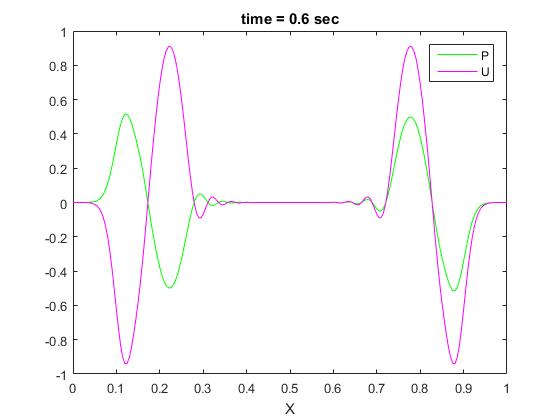
\includegraphics[width=0.3\textwidth]{fig/p1/sin_0p6.jpg}}
   \subfloat [0.8 sec]{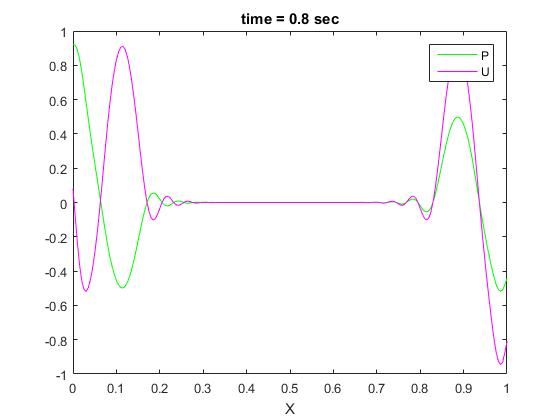
\includegraphics[width=0.3\textwidth]{fig/p1/sin_0p8.jpg}}
   \subfloat [1 sec]{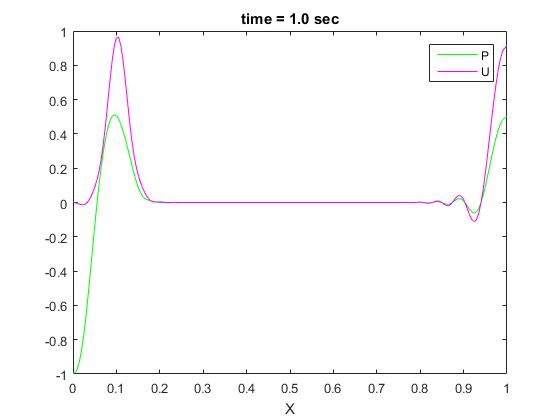
\includegraphics[width=0.3\textwidth]{fig/p1/sin_1.jpg}}
   
   
   \subfloat [1.6 sec]{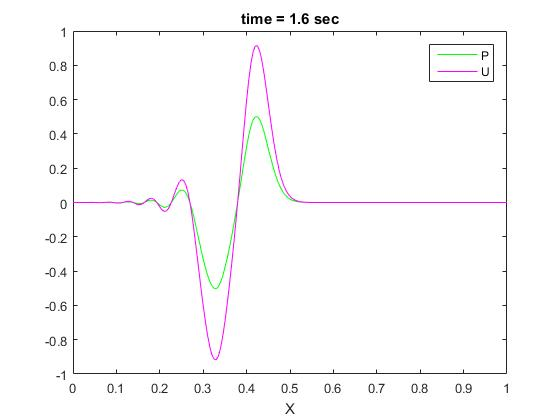
\includegraphics[width=0.3\textwidth]{fig/p1/sin_1p6.jpg}}
   \subfloat [2.2 sec]{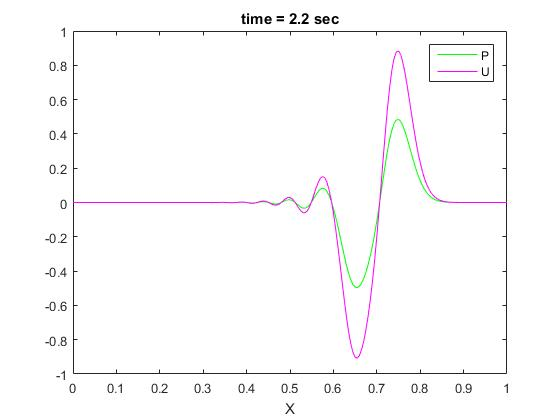
\includegraphics[width=0.3\textwidth]{fig/p1/sin_2p2.jpg}}
   \subfloat [4 sec]{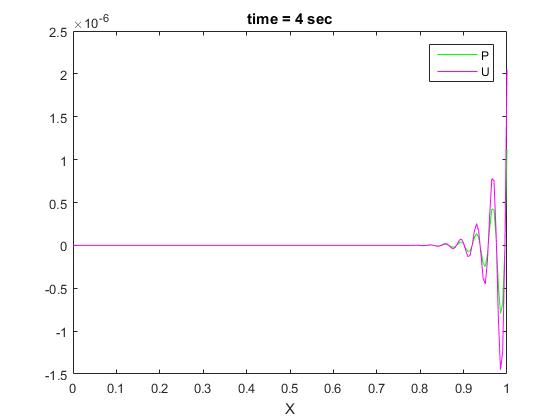
\includegraphics[width=0.3\textwidth]{fig/p1/sin_4.jpg}}
   
     \caption{Solution of the linearized equations of acoustics using \protect{\lw} method on cell-centered grid with sine wave as initial condition for the pressure and zero initial condition for the speed at different time intervals.}
   \label{fig:sol_sin}
\end{figure} 

\begin{figure}[]
 \centering     
   \subfloat [0 sec]{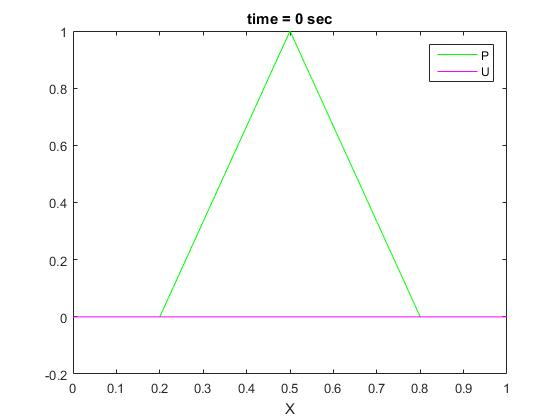
\includegraphics[width=0.3\textwidth]{fig/p1/tri_0.jpg}}
   \subfloat [0.2 sec]{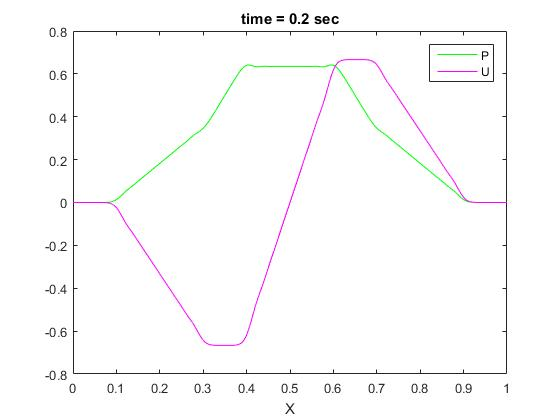
\includegraphics[width=0.3\textwidth]{fig/p1/tri_0p2.jpg}}
   \subfloat [0.4 sec]{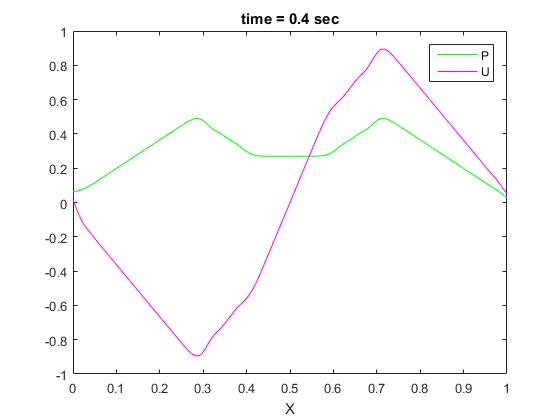
\includegraphics[width=0.3\textwidth]{fig/p1/tri_0p4.jpg}}
   
   \subfloat [0.6 sec]{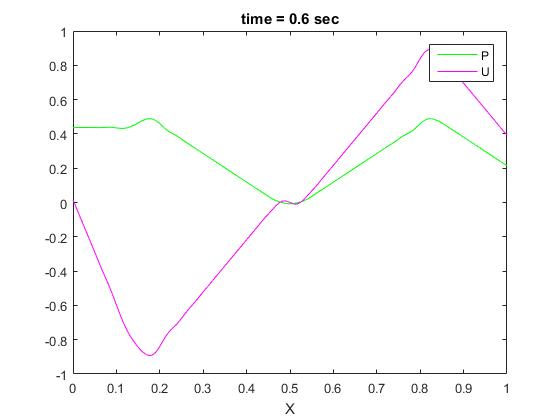
\includegraphics[width=0.3\textwidth]{fig/p1/tri_0p6.jpg}}
   \subfloat [0.8 sec]{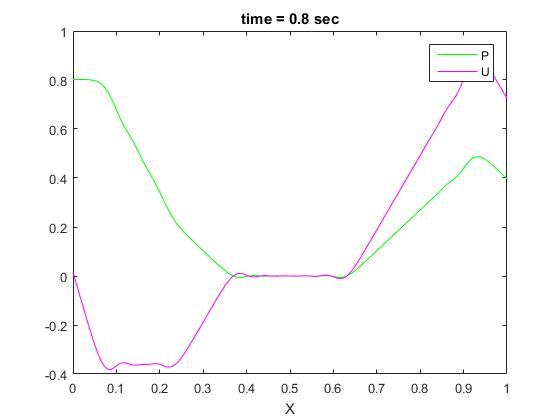
\includegraphics[width=0.3\textwidth]{fig/p1/tri_0p8.jpg}}
   \subfloat [1 sec]{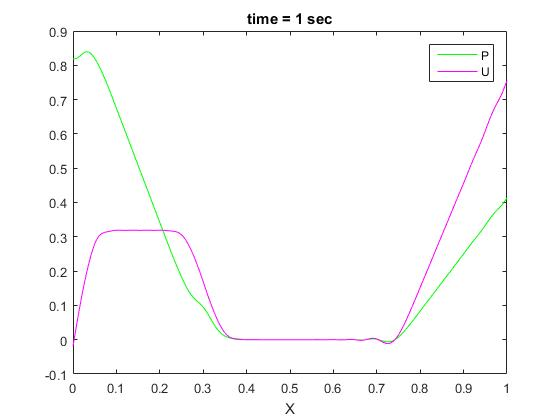
\includegraphics[width=0.3\textwidth]{fig/p1/tri_1.jpg}}
  
     \subfloat [1.6 sec]{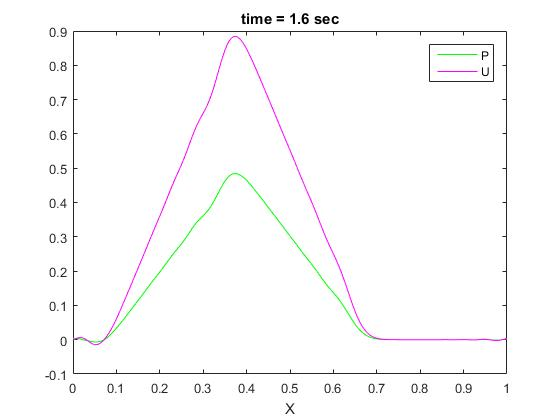
\includegraphics[width=0.3\textwidth]{fig/p1/tri_1p6.jpg}}
   \subfloat [2.2 sec]{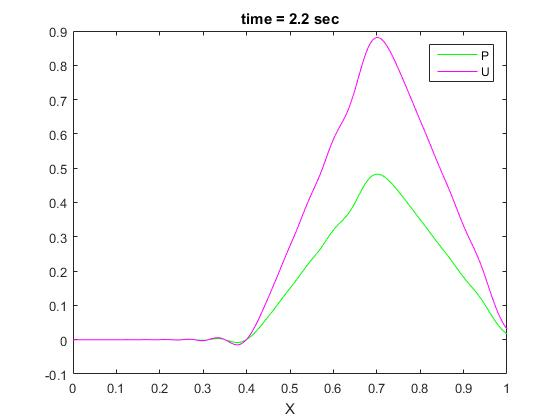
\includegraphics[width=0.3\textwidth]{fig/p1/tri_2p2.jpg}}
   \subfloat [4 sec]{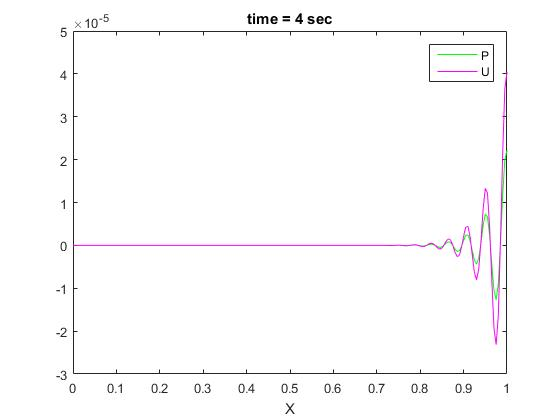
\includegraphics[width=0.3\textwidth]{fig/p1/tri_4.jpg}} 
     \caption{Solution of the linearized equations of acoustics using \protect{\lw} method on cell-centered grid triangular function as initial condition for the pressure and zero initial condition for the speed at different time intervals.}
   \label{fig:sol_tri}
\end{figure} 
      
\begin{figure}[]
 \centering     
   \subfloat [0 sec]{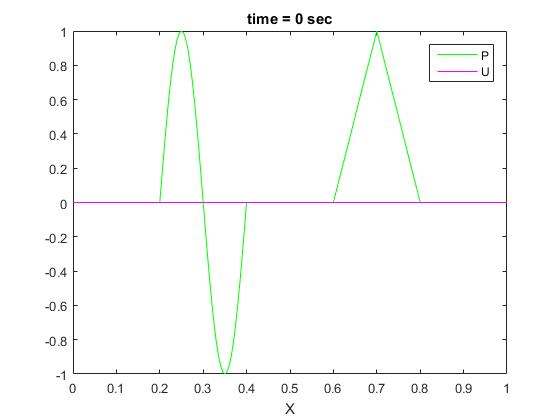
\includegraphics[width=0.3\textwidth]{fig/p1/sin_tri_0.jpg}}
   \subfloat [0.2 sec]{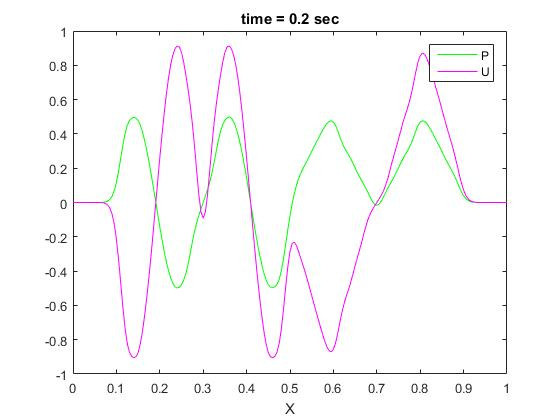
\includegraphics[width=0.3\textwidth]{fig/p1/sin_tri_0p2.jpg}}
   \subfloat [0.4 sec]{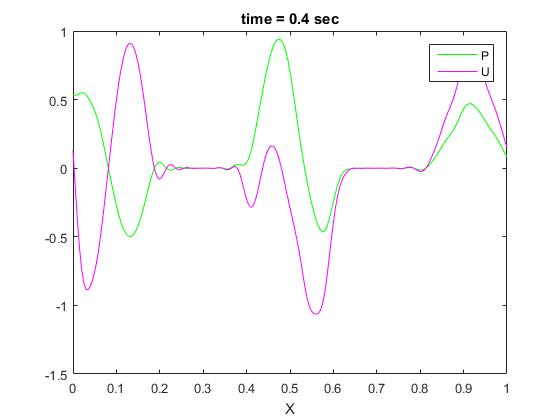
\includegraphics[width=0.3\textwidth]{fig/p1/sin_tri_0p4.jpg}}
   
   \subfloat [0.6 sec]{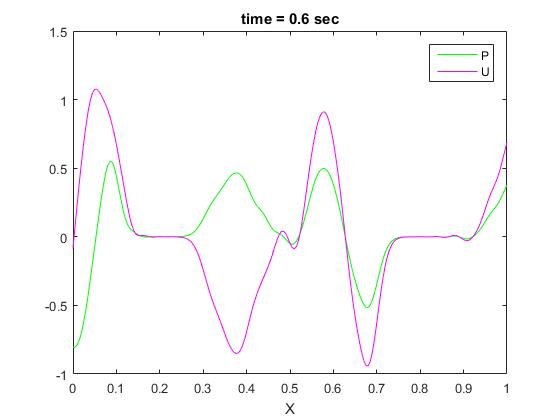
\includegraphics[width=0.3\textwidth]{fig/p1/sin_tri_0p6.jpg}}
   \subfloat [0.8 sec]{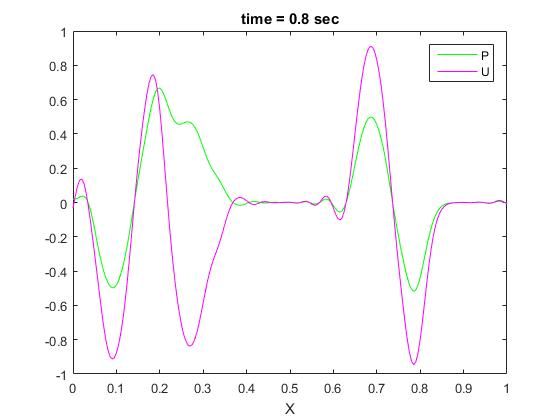
\includegraphics[width=0.3\textwidth]{fig/p1/sin_tri_0p8.jpg}}
   \subfloat [1 sec]{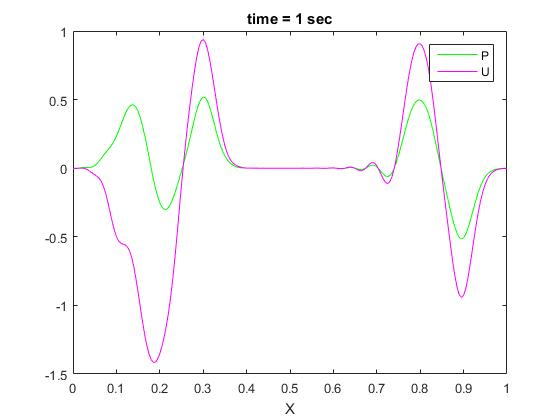
\includegraphics[width=0.3\textwidth]{fig/p1/sin_tri_1.jpg}}

   \subfloat [1.6 sec]{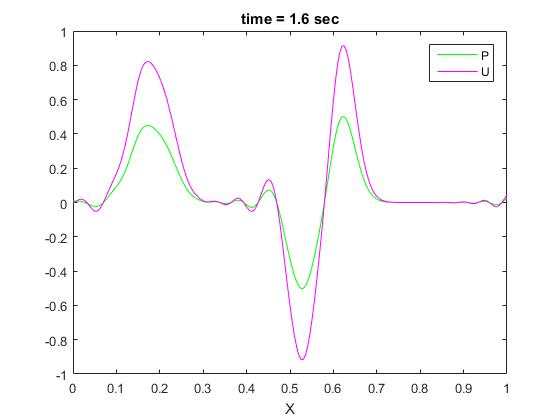
\includegraphics[width=0.3\textwidth]{fig/p1/sin_tri_1p6.jpg}}
   \subfloat [2.2 sec]{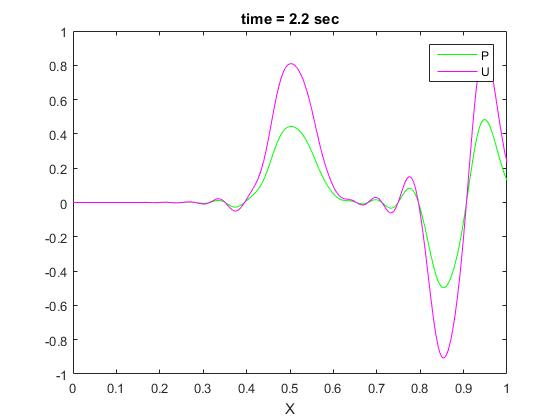
\includegraphics[width=0.3\textwidth]{fig/p1/sin_tri_2p2.jpg}}
   \subfloat [4 sec]{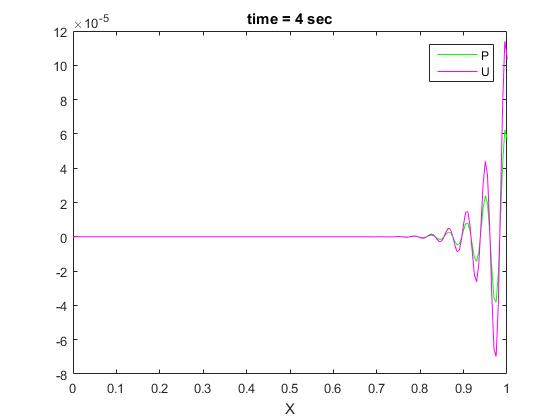
\includegraphics[width=0.3\textwidth]{fig/p1/sin_tri_4.jpg}}      
     \caption{Solution of the linearized equations of acoustics using \protect{\lw} method on cell-centered grid with mixed sine wave and triangular function as initial condition for the pressure and zero initial condition for the speed at different time intervals.}
   \label{fig:sol_sin_tri}
\end{figure} 

\begin{figure}[]
 \centering     
   \subfloat [0 sec]{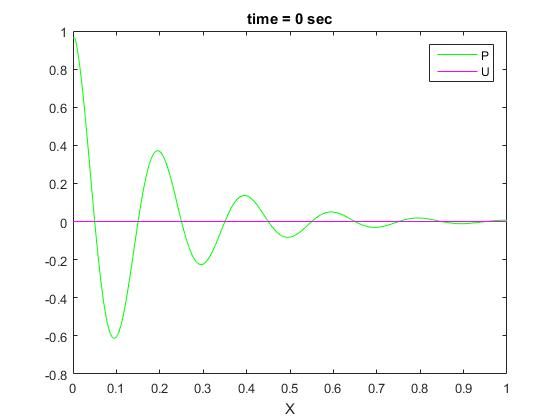
\includegraphics[width=0.3\textwidth]{fig/p1/sin_expo_0.jpg}}
   \subfloat [0.2 sec]{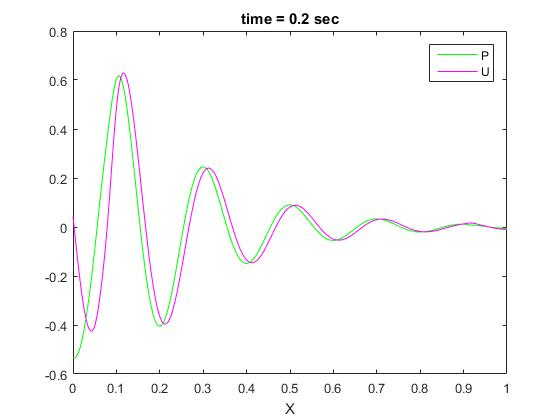
\includegraphics[width=0.3\textwidth]{fig/p1/sin_expo_0p2.jpg}}
   \subfloat [0.4 sec]{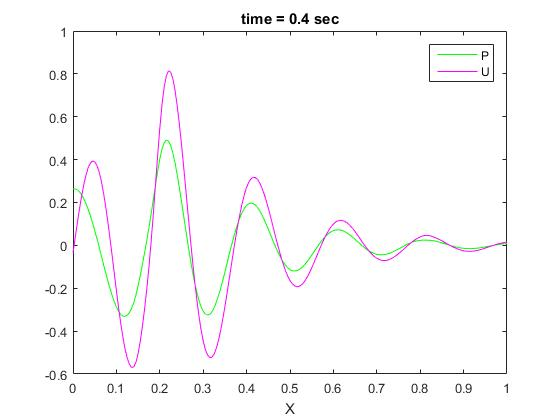
\includegraphics[width=0.3\textwidth]{fig/p1/sin_expo_0p4.jpg}}
   
   \subfloat [0.6 sec]{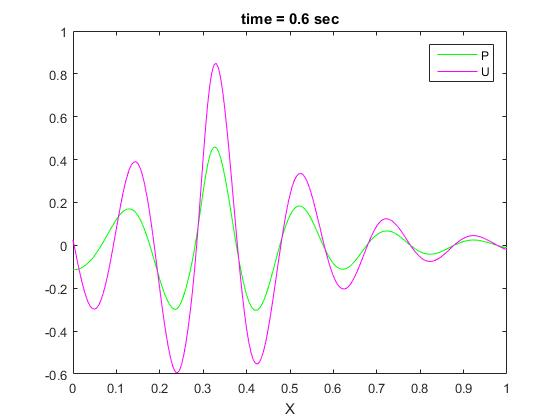
\includegraphics[width=0.3\textwidth]{fig/p1/sin_expo_0p6.jpg}}
   \subfloat [0.8 sec]{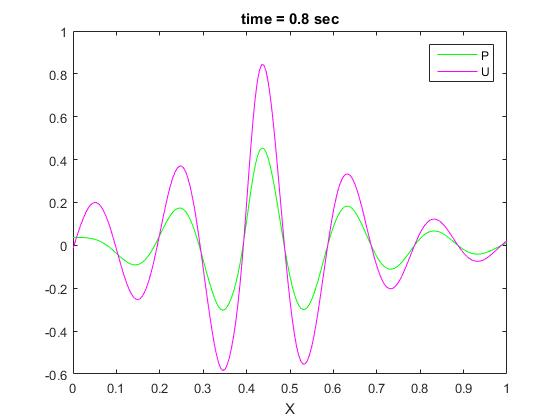
\includegraphics[width=0.3\textwidth]{fig/p1/sin_expo_0p8.jpg}}
   \subfloat [1 sec]{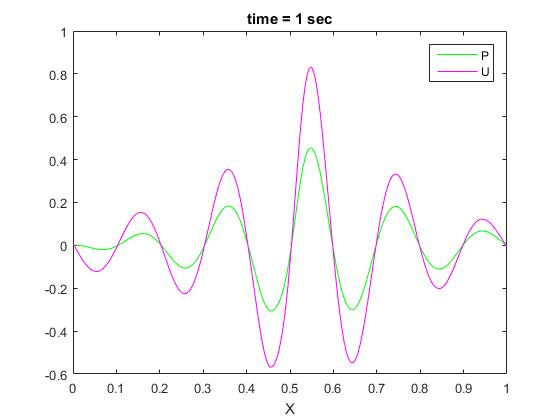
\includegraphics[width=0.3\textwidth]{fig/p1/sin_expo_1.jpg}}

   \subfloat [1.6 sec]{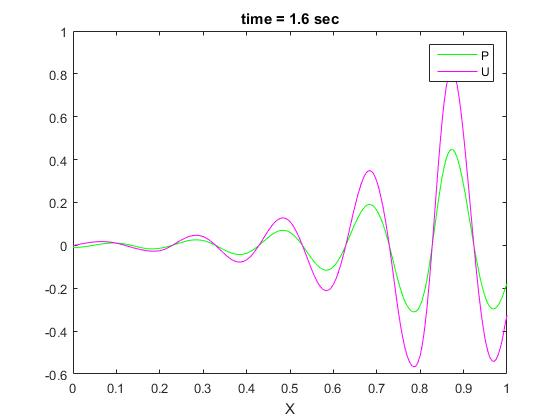
\includegraphics[width=0.3\textwidth]{fig/p1/sin_expo_1p6.jpg}}
   \subfloat [2.2 sec]{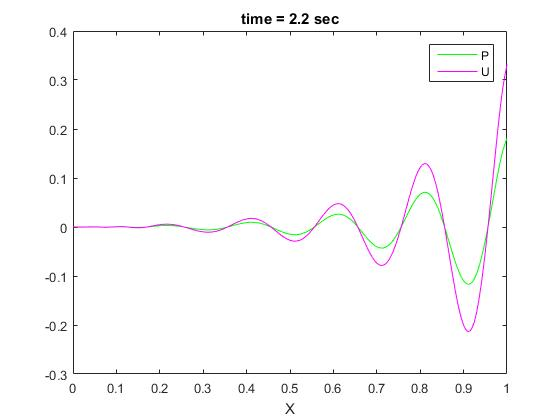
\includegraphics[width=0.3\textwidth]{fig/p1/sin_expo_2p2.jpg}}
   \subfloat [4 sec]{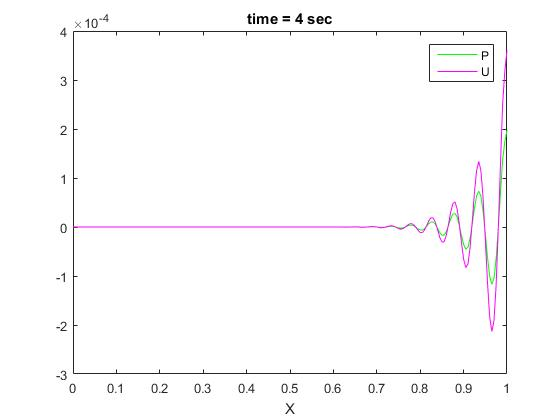
\includegraphics[width=0.3\textwidth]{fig/p1/sin_expo_4.jpg}}   
     \caption{Solution of the linearized equations of acoustics using \protect{\lw} method on cell-centered grid with decaying exponential sine wave as initial condition for the pressure and zero initial condition for the speed at different time intervals.}
   \label{fig:sol_sin_expo}
\end{figure} 


\paragraph{Part 3:} 
The boundary conditions given on the left wall has zero pressure gradient and the velocity is zero (since the right and left cells has the same value with opposite signs). This means that the momentum of the sound wave is preserved and thus it bounces back and no sound it transmitted through the wall. On the right boundary, since the velocity and pressure has positive values and due to their momentum, they will continue travel in this same direction (and not bounce back). 

